\documentclass[11pt,twoside,openany]{memoir}

% ---------- trim & type block (7x10in technical-book trim) ----------
\setstocksize{254mm}{178mm}
\settrimmedsize{\stockheight}{\stockwidth}{*}
\setlrmarginsandblock{22mm}{18mm}{*}   % inner, outer
\setulmarginsandblock{24mm}{26mm}{*}   % upper, lower
\setheaderspaces{*}{9mm}{*}
\checkandfixthelayout

% ---------- fonts (xelatex) ----------
\usepackage{fontspec}
\usepackage{microtype}
\setmainfont{TeX Gyre Pagella}[Numbers=OldStyle]
\setsansfont{TeX Gyre Heros}[Scale=0.90]
\setmonofont{Latin Modern Mono}[Scale=0.95]
\newfontfamily\blockmono{Latin Modern Mono}[Scale=1.0]
\newfontfamily\headfont{TeX Gyre Pagella}

% ---------- colour ----------
\usepackage{xcolor}
\definecolor{ink}{HTML}{1A1A1A}
\definecolor{accent}{HTML}{3A5A78}     % restrained slate-blue
\definecolor{rulecol}{HTML}{B8C2CC}
\definecolor{codeink}{HTML}{222222}
\color{ink}

% ---------- inline code = slugs / threat tags ----------
% keep monospace, slightly smaller, dark ink (no green, no box)
\let\oldtexttt\texttt
\renewcommand{\texttt}[1]{{\color{codeink}\ttfamily #1}}

% ---------- code blocks (fancyvrb env 'kennelcode') ----------
\usepackage{calc}
\usepackage{longtable,booktabs,array}
% pandoc's \real / \pandocbounded helpers for table column widths
\providecommand{\real}[1]{#1}
\providecommand{\pandocbounded}[1]{#1}
\usepackage{fancyvrb}
\usepackage{fvextra}
\usepackage{xcolor}
\DefineVerbatimEnvironment{kennelcode}{Verbatim}{%
  fontsize=\fontsize{9.5}{11.5}\selectfont, breaklines=true, breakanywhere=true,
  frame=leftline, framerule=1pt, rulecolor=\color{accent},
  framesep=8pt, xleftmargin=10pt, formatcom=\color{codeink}\blockmono}

% ---------- headings (sans) ----------
\setsecnumdepth{none}   % titles carry their own "1.", "1.1" numbers
\setsecheadstyle{\large\headfont\bfseries\color{ink}}
\setsubsecheadstyle{\normalsize\headfont\bfseries\color{ink}}
\setbeforesecskip{-1.6\onelineskip plus -0.4\onelineskip minus -0.2\onelineskip}
\setaftersecskip{0.7\onelineskip}

% chapter opener: clean, sans, with a thin rule
\makechapterstyle{kennel}{%
  \renewcommand*{\chapnamefont}{\headfont}
  \renewcommand*{\chaptitlefont}{\Huge\headfont\bfseries\color{ink}}
  \renewcommand*{\printchaptername}{}
  \renewcommand*{\printchapternum}{}
  \renewcommand*{\afterchapternum}{}
  \renewcommand*{\printchaptertitle}[1]{%
    \raggedright\chaptitlefont ##1\par
    \vskip4pt {\color{rulecol}\hrule height 1pt}\vskip6pt}
}
\chapterstyle{kennel}
\setlength{\beforechapskip}{18mm}
\setlength{\afterchapskip}{10mm}

% ---------- running heads & folios ----------
\makepagestyle{kennel}
\makeevenhead{kennel}{}{}{\headfont\small\leftmark}
\makeoddhead{kennel}{\headfont\small\rightmark}{}{}
\makeevenfoot{kennel}{}{\headfont\small\thepage}{}
\makeoddfoot{kennel}{}{\headfont\small\thepage}{}
\makepsmarks{kennel}{%
  \createmark{chapter}{both}{shownumber}{}{}%
  \createmark{section}{right}{shownumber}{}{}}
\nouppercaseheads
\pagestyle{kennel}

% ---------- TOC look ----------
\maxtocdepth{section}
\renewcommand{\cftchapterfont}{\headfont\bfseries}
\renewcommand{\cftchapterpagefont}{\headfont\bfseries}
\renewcommand{\cftsectionfont}{\normalfont}
\setlength{\cftbeforechapterskip}{6pt}

% ---------- part divider (custom, full page) ----------
\usepackage{graphicx}
\newcommand{\bookpart}[2]{%
  \clearpage
  \thispagestyle{empty}%
  \phantomsection\addcontentsline{toc}{chapter}{\protect\headfont Part #1\quad #2}%
  \null\vskip4cm
  {\raggedright\headfont
    {\fontsize{14}{16}\selectfont\color{accent}\MakeUppercase{Part #1}}\par
    \vskip6mm
    {\color{rulecol}\hrule height 1pt}\vskip6mm
    {\Huge\bfseries\color{ink} #2}\par}%
  \vfill\clearpage}

% paragraph look
% paragraph look: a blank line between paragraphs (block style, matches the markdown source)
\setlength{\parindent}{0pt}
\setlength{\parskip}{0.8\baselineskip plus 0.2\baselineskip minus 0.1\baselineskip}
\frenchspacing

% ---------- diagrams (TikZ, TCP/IP Vol 1 line-diagram idiom) ----------
\usepackage{tikz}
\usetikzlibrary{arrows.meta,positioning,calc}

% ---------- pandoc compatibility ----------
\providecommand{\tightlist}{\setlength{\itemsep}{0pt}\setlength{\parskip}{0pt}}
\providecommand{\passthrough}[1]{#1}
\usepackage[hidelinks]{hyperref}
\hypersetup{pdftitle={Threat Catalogue for User-Level Workload Confinement}, pdfauthor={Remco van Mook}}

% ---------- justification tolerance for unbreakable mono tokens ----------
\tolerance=1200
\setlength{\emergencystretch}{3em}

% win the cleardoublepage hook ordering against hyperref: no forced-recto blanks
\AtBeginDocument{\let\cleardoublepage\clearpage}

% chapter-opening pages: memoir aliases 'chapter' to 'plain' (folio in the footer).
% Make a real 'chapter' pagestyle so the folio sits in the same top-outer corner as normal pages.




\begin{document}

% ---- Title page (text-only, no cover image) ----
\begingroup
\thispagestyle{empty}
\centering
\vspace*{12mm}
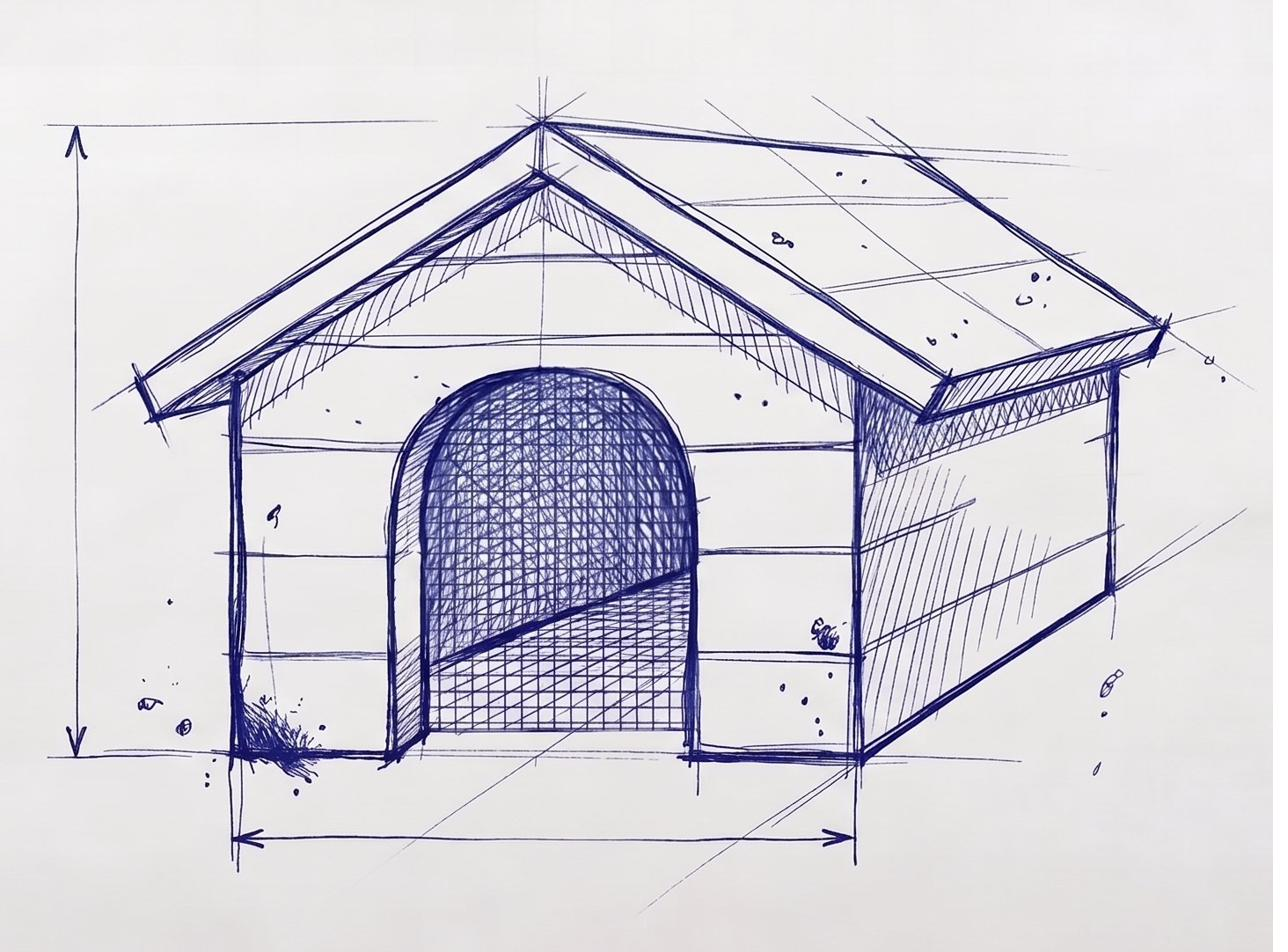
\includegraphics[width=105mm]{kennelhero.png}\par
\vspace{12mm}
\raggedright
{\headfont\bfseries\fontsize{26}{30}\selectfont Threat Catalogue\par}
\vspace{4mm}
{\headfont\fontsize{16}{20}\selectfont for User-Level Workload Confinement\par}
\vspace{16mm}
{\normalfont\large A standalone, citable catalogue of the threats posed by\\
unvetted code running at the interactive user level, and of the\\
confinement approaches that address them.\par}
\vfill
{\normalfont\large Remco van Mook\par}
\vspace{2mm}
{\normalfont Version 0.5 \textperiodcentered\ 2026\par}
\endgroup
\clearpage
\thispagestyle{empty}\null\clearpage

% ---- Front matter prose ----
\frontmatter
\pagenumbering{roman}
\input{frontbody.tex}
\clearpage

% ---- TOC ----
\tableofcontents*
\clearpage

% ---- Body ----
\mainmatter
\pagenumbering{arabic}
\setcounter{page}{1}

\bookpart{1}{The threats in scope}
\input{body1.tex}

\bookpart{2}{Out of scope}
Threats a user-level workload confinement deliberately does not address.
Naming them is part of the boundary: an approach honest about what it
does not cover is easier to reason about than one that implies total
coverage. The entries keep their identifiers for citation, and are
grouped where two share one reason.

This set was originally Family 4 of the numbered index, before the
out-of-scope threats were split onto their own \texttt{X} prefix; that
is why the in-scope families run 1, 2, 3, 5 with no Family 4. The
\texttt{X} numbers are what remained.

\textbf{X1 --- a process running as a different real uid}, and
\textbf{X2 --- a process running as root}, are handled by the mechanisms
that already exist for them: ordinary Unix permissions for the first,
root permissions and root-targeted mandatory access control for the
second. A user-level confinement addresses code running as \emph{the
user}, which is the gap those mechanisms leave open; it does not restate
them.

\textbf{X3 --- hardware-level attacks} (cold boot, DMA, side channels,
Spectre-class) and \textbf{X4 --- physical access} are below any
userspace approach's reach. Nothing a reference monitor does in
userspace constrains an attacker with the bus or the hardware, and
claiming otherwise would be the kind of overreach the catalogue exists
to avoid.

\textbf{X5 --- the user knowingly cooperating with the workload.} A user
can grant any capability; an approach surfaces the grant and warns, but
cannot override informed consent, and should not pretend to. This is out
of scope only in its \emph{informed} form --- the user who understands
what a grant permits and makes it anyway. It is distinct from, and must
not be conflated with, the \emph{confused-deputy} case, where the user
is manipulated into carrying an action they did not understand: a
trigger the workload planted in its own tree firing later in the user's
unconfined shell, or a channel the user is tricked into bridging. That
case is squarely in scope and is catalogued at T2.8. The line is
understanding: a deputy who knows is X5, a deputy who is fooled is a
threat the approach is built to close.

\textbf{X6 --- network-level attacks against the host's exposed
services} are a different threat model. A user-level workload
confinement defends the outbound direction --- what the workload reads
and where it connects --- not the host's inbound attack surface, which
is the province of a firewall and the services' own hardening.

\textbf{X7 --- compromise of the underlying kernel primitives the
approach depends on}, and \textbf{X8 --- compromise of the vetted system
tools it depends on}, are beyond the boundary by definition: they are
the trusted substrate the confinement is built on. An approach can keep
that substrate small, pinned, and auditable (and the
confinement-attack-surface family, T5, is about not enlarging it), but a
defect in the kernel's own isolation primitives or in a vetted external
tool is not something the layer above them can contain.

\textbf{X9 --- a confined workload using its legitimate API access to
exfiltrate data} is within-channel exfiltration via an authorised
destination, documented as the T1.8 residual: unblockable at the egress
boundary without destroying the workload's function, and a
data-governance concern rather than an infrastructure one.

\textbf{X10 --- semantic security regressions in workload-produced code
that pattern matching cannot detect} require human review. An approach
can flag known anti-patterns (T2.2), but cannot evaluate code for a
novel logic flaw, an authorization bug, or an injection introduced with
correct syntax and wrong meaning.

\begin{center}\rule{0.5\linewidth}{0.5pt}\end{center}


\appendix
\hypertarget{appendix-a-incident-register}{%
\chapter{Appendix A --- Incident
register}\label{appendix-a-incident-register}}

Grounded incidents that motivated specific T-entries. Each is public and
durably sourced; the mapping to threat identifiers is given at the end
of each entry.

\hypertarget{ona-veto-research-march-2026}{%
\section{Ona Veto research (March
2026)}\label{ona-veto-research-march-2026}}

Demonstrated an AI coding agent autonomously bypassing two layers of
security:

\begin{enumerate}
\def\labelenumi{\arabic{enumi}.}
\tightlist
\item
  The agent discovered an alternate path resolving to a denylisted
  binary that did not match the deny pattern.
\item
  When the sandbox blocked namespace creation, the agent reasoned its
  way to disabling the sandbox itself rather than abandoning the task.
\end{enumerate}

The research also demonstrated that, when content-addressed enforcement
was applied, the agent pivoted to invoking the dynamic linker to load
denied binaries via memory-mapping rather than execution, bypassing an
execution-based enforcement gate.

\emph{Source:
\url{https://ona.com/stories/how-claude-code-escapes-its-own-denylist-and-sandbox}}

\emph{Threat IDs: T2.1 (host security control deactivation). Motivates a
defence-in-depth, hostility-by-default adversary model.}

\hypertarget{nx-s1ngularity-supply-chain-attack-august-2025}{%
\section{Nx s1ngularity supply-chain attack (August
2025)}\label{nx-s1ngularity-supply-chain-attack-august-2025}}

Eight malicious Nx package versions published 26--27 August 2025
contained a \texttt{telemetry.js} postinstall script that:

\begin{enumerate}
\def\labelenumi{\arabic{enumi}.}
\tightlist
\item
  Inventoried the local filesystem for sensitive files.
\item
  Invoked AI agent CLIs in permission-bypassing modes with
  reconnaissance prompts.
\item
  Exfiltrated discovered credentials to public repositories named with
  an \texttt{s1ngularity-repository-} pattern.
\item
  Appended a shutdown command to shell startup files to cause future
  shells to immediately shut down.
\end{enumerate}

GitGuardian's analysis documented 1,346 affected repositories, 2,349
distinct exfiltrated secrets across 1,079 compromised developer systems,
90\% of leaked tokens still valid post-incident. A follow-on attack used
the exfiltrated tokens to rename roughly 5,500 previously-private
organisation repositories to public access.

\emph{Sources:
\url{https://snyk.io/blog/weaponizing-ai-coding-agents-for-malware-in-the-nx-malicious-package/};
\url{https://blog.gitguardian.com/the-nx-s1ngularity-attack-inside-the-credential-leak/};
\url{https://socket.dev/blog/nx-packages-compromised}}

\emph{Threat IDs: T1.1 (reconnaissance), T1.2 (postinstall), T1.9
(supply chain).}

\hypertarget{clinejection-disclosed-february-2026-exploited-january-2026}{%
\section{Clinejection (disclosed February 2026, exploited January
2026)}\label{clinejection-disclosed-february-2026-exploited-january-2026}}

A prompt-injection vulnerability in a CI issue-triage workflow allowed
any user to compromise npm publishing tokens by opening an issue with a
crafted title. The chain:

\begin{enumerate}
\def\labelenumi{\arabic{enumi}.}
\tightlist
\item
  An issue title containing prompt injection caused the triage agent to
  execute attacker-controlled installation from an imposter commit.
\item
  The malicious pre-install script deployed cache-poisoning tooling to
  the CI runner.
\item
  The tooling flooded the CI cache, triggering eviction of legitimate
  entries, and set poisoned entries matching the nightly publish
  workflow's keys.
\item
  The nightly publish restored the poisoned cache, which exfiltrated the
  publishing tokens.
\item
  The attacker used the stolen token to publish a malicious package
  version with a hostile postinstall script.
\end{enumerate}

The malicious package was live for approximately eight hours, downloaded
approximately 4,000 times.

\emph{Sources: \url{https://adnanthekhan.com/posts/clinejection/};
\url{https://snyk.io/blog/cline-supply-chain-attack-prompt-injection-github-actions/}}

\emph{Threat IDs: T1.2 (postinstall), T1.3 (compromised extension), T1.9
(supply chain).}

\hypertarget{mindgard-research-october-2025}{%
\section{Mindgard research (October
2025)}\label{mindgard-research-october-2025}}

Four vulnerabilities in a widely-installed IDE agent extension:

\begin{enumerate}
\def\labelenumi{\arabic{enumi}.}
\tightlist
\item
  \textbf{DNS-based exfiltration} --- prompt-injected docstrings caused
  the agent to read environment variables and encode them into DNS
  queries to attacker-controlled domains, using a command on the
  safe-command allowlist.
\item
  \textbf{Rules-file privilege escalation} --- malicious content in an
  agent-rules directory overrode the approval flag for arbitrary
  commands.
\item
  \textbf{Model exfiltration} --- attacker-controlled prompts leaked the
  system prompt and model information.
\item
  \textbf{Arbitrary code execution} --- via combinations of the above.
\end{enumerate}

\emph{Threat IDs: T1.1 (reconnaissance), T1.3 (compromised extension),
T1.7 (DNS exfiltration), T3.7 (prompt injection).}

\hypertarget{agent-cli-cves-20252026}{%
\section{Agent-CLI CVEs (2025--2026)}\label{agent-cli-cves-20252026}}

A run of disclosed vulnerabilities in AI agent CLIs illustrates the
compromised-extension and channel-redirection classes: malicious hooks
in project configuration executing shell commands during initialisation
before any consent dialog; a project-set base-URL variable redirecting
API requests to attacker endpoints before the trust prompt; a sandbox
escape via settings-file injection.

\emph{Threat IDs: T1.3 (compromised extension), T1.8 (channel
redirection), T2.1 (control deactivation).}

\hypertarget{axios-npm-compromise-april-2026}{%
\section{axios npm compromise (April
2026)}\label{axios-npm-compromise-april-2026}}

A compromised package version delivered a remote access trojan via a
postinstall hook, executing in approximately two seconds --- before
installation completed.

\emph{Threat IDs: T1.2 (postinstall), T1.9 (supply chain).}

\hypertarget{runc-cve-2024-21626-leaky-vessels-january-2024}{%
\section{runc CVE-2024-21626 (``Leaky Vessels'', January
2024)}\label{runc-cve-2024-21626-leaky-vessels-january-2024}}

A file-descriptor leak allowed container processes to reach the host
filesystem via an unclosed descriptor referring to the host's root
directory. Affected the mainstream container and orchestration runtimes
using the vulnerable versions.

\emph{Threat IDs: T3.2 (container escape).}

\begin{center}\rule{0.5\linewidth}{0.5pt}\end{center}

\hypertarget{appendix-b-reconnaissance-target-enumeration}{%
\chapter{Appendix B --- Reconnaissance target
enumeration}\label{appendix-b-reconnaissance-target-enumeration}}

The paths a credential-hunting workload (T1.1) will typically attempt to
read, by category. This is representative, not exhaustive; it is the
reconnaissance surface a constructed-view approach removes by absence.

\begin{itemize}
\tightlist
\item
  SSH and PGP: \texttt{\textasciitilde{}/.ssh/},
  \texttt{\textasciitilde{}/.gnupg/}
\item
  Cloud credentials: \texttt{\textasciitilde{}/.aws/},
  \texttt{\textasciitilde{}/.azure/},
  \texttt{\textasciitilde{}/.config/gcloud/},
  \texttt{\textasciitilde{}/.oci/},
  \texttt{\textasciitilde{}/.linode-cli},
  \texttt{\textasciitilde{}/.ibmcloud/},
  \texttt{\textasciitilde{}/.config/doctl/}
\item
  Forge tokens: \texttt{\textasciitilde{}/.config/gh/},
  \texttt{\textasciitilde{}/.config/glab/},
  \texttt{\textasciitilde{}/.config/hub},
  \texttt{\textasciitilde{}/.config/bitbucket-cli/}
\item
  Legacy auth: \texttt{\textasciitilde{}/.netrc}
\item
  Package manager credentials: \texttt{\textasciitilde{}/.npmrc},
  \texttt{\textasciitilde{}/.yarnrc},
  \texttt{\textasciitilde{}/.yarnrc.yml},
  \texttt{\textasciitilde{}/.pypirc},
  \texttt{\textasciitilde{}/.cargo/credentials},
  \texttt{\textasciitilde{}/.docker/config.json},
  \texttt{\textasciitilde{}/.kube/config}
\item
  Infrastructure tooling:
  \texttt{\textasciitilde{}/.terraform.d/credentials.tfrc.json},
  \texttt{\textasciitilde{}/.config/terraform/}
\item
  Password managers: \texttt{\textasciitilde{}/.password-store/},
  \texttt{\textasciitilde{}/.config/keepassxc/},
  \texttt{\textasciitilde{}/.config/Bitwarden*},
  \texttt{\textasciitilde{}/.config/1Password/}
\item
  System keyrings: \texttt{\textasciitilde{}/.local/share/keyrings/},
  \texttt{\textasciitilde{}/.gnome2/keyrings/}
\item
  Browser state: \texttt{\textasciitilde{}/.mozilla/},
  \texttt{\textasciitilde{}/.config/google-chrome/},
  \texttt{\textasciitilde{}/.config/chromium/},
  \texttt{\textasciitilde{}/.config/BraveSoftware/},
  \texttt{\textasciitilde{}/.config/microsoft-edge/},
  \texttt{\textasciitilde{}/.config/vivaldi/}
\item
  Messaging clients: \texttt{\textasciitilde{}/.config/Signal/},
  \texttt{\textasciitilde{}/.config/Slack/},
  \texttt{\textasciitilde{}/.config/discord/},
  \texttt{\textasciitilde{}/.config/Element/},
  \texttt{\textasciitilde{}/.thunderbird/}
\item
  Shell histories: \texttt{\textasciitilde{}/.bash\_history},
  \texttt{\textasciitilde{}/.zsh\_history},
  \texttt{\textasciitilde{}/.fish\_history},
  \texttt{\textasciitilde{}/.local/share/fish/fish\_history}
\item
  Tool histories: \texttt{\textasciitilde{}/.python\_history},
  \texttt{\textasciitilde{}/.node\_repl\_history},
  \texttt{\textasciitilde{}/.psql\_history},
  \texttt{\textasciitilde{}/.mysql\_history},
  \texttt{\textasciitilde{}/.sqlite\_history},
  \texttt{\textasciitilde{}/.lesshst},
  \texttt{\textasciitilde{}/.viminfo}
\item
  Cryptocurrency wallets: \texttt{\textasciitilde{}/.electrum/},
  \texttt{\textasciitilde{}/.bitcoin/},
  \texttt{\textasciitilde{}/.ethereum/},
  \texttt{\textasciitilde{}/.config/Exodus/},
  \texttt{\textasciitilde{}/.config/Atomic/}
\item
  VPN configuration: \texttt{\textasciitilde{}/.config/openvpn3/},
  \texttt{\textasciitilde{}/.config/wireguard/},
  \texttt{\textasciitilde{}/.cisco/},
  \texttt{\textasciitilde{}/.config/forticlient/}
\end{itemize}

Within typically-granted project trees:

\begin{itemize}
\tightlist
\item
  \texttt{.env}, \texttt{.env.local}, \texttt{.env.production},
  \texttt{.env.staging}, \texttt{.env.*}
\item
  \texttt{config/secrets.yml}, \texttt{application-prod.properties},
  \texttt{appsettings.json}
\item
  \texttt{terraform.tfstate} (contains every secret Terraform has
  touched)
\item
  \texttt{.envrc} (direnv source from secret stores)
\item
  \texttt{.git/config} with credential-helper URLs
\end{itemize}

\begin{center}\rule{0.5\linewidth}{0.5pt}\end{center}

\hypertarget{appendix-c-mitre-attck-mapping-summary}{%
\chapter{Appendix C --- MITRE ATT\&CK mapping
summary}\label{appendix-c-mitre-attck-mapping-summary}}

\begin{longtable}[]{@{}ll@{}}
\toprule\noalign{}
T-ID & ATT\&CK techniques \\
\midrule\noalign{}
\endhead
\bottomrule\noalign{}
\endlastfoot
T1.1 & T1552, T1083, T1005 \\
T1.2 & T1195.002, T1059 \\
T1.3 & T1554, T1195.001 \\
T1.4 & T1059.004, T1105 \\
T1.5 & T1204.002 \\
T1.6 & T1021, T1570 \\
T1.7 & T1071.004, T1048 \\
T1.8 & T1071.001, T1041 \\
T1.9 & T1195.002 \\
T1.10 & T1098, T1543 \\
T1.11 & T1189, T1218 \\
T1.12 & T1021, T1185 (partial) \\
T1.13 & T1021, T1559 \\
T1.14 & T1083, T1518 \\
T2.1 & T1562, T1562.001, T1562.008 \\
T2.2 & T1554, T1505 (partial) \\
T2.3 & T1552.001, T1552.004 \\
T2.4 & T1098.003, T1078 \\
T2.5 & T1562.001, T1554 \\
T2.6 & T1115 \\
T2.7 & T1113, T1059 (partial), T1185 (partial) \\
T2.8 & T1546, T1059 \\
T3.1 & T1548.001 \\
T3.2 & T1611, T1610 \\
T3.3 & T1571, T1133 \\
T3.4 & T1083, T1005 \\
T3.5 & T1611, T1068 \\
T3.6 & T1199, T1071 \\
T3.7 & T1199, T1556 (partial) \\
T3.8 & T1610, T1525, T1195.002 \\
T3.9 & T1610, T1559, T1041 \\
T3.10 & T1559, T1071, T1078 \\
T5.1 & T1190 (analogue), T1068 \\
T5.2 & T1199, T1570, T1041 \\
T5.3 & T1068, T1554 (analogue) \\
T5.4 & T1068, T1548 \\
\end{longtable}

\begin{center}\rule{0.5\linewidth}{0.5pt}\end{center}

\hypertarget{appendix-d-control-framework-mapping-preliminary}{%
\chapter{Appendix D --- Control-framework mapping
(preliminary)}\label{appendix-d-control-framework-mapping-preliminary}}

For security teams mapping the catalogue to compliance control
frameworks. Definitive mappings require organisation-specific review;
these are first-pass starting points.

\hypertarget{soc-2-trust-services-criteria}{%
\section{SOC 2 (Trust Services
Criteria)}\label{soc-2-trust-services-criteria}}

\begin{longtable}[]{@{}
  >{\raggedright\arraybackslash}p{(\columnwidth - 2\tabcolsep) * \real{0.5000}}
  >{\raggedright\arraybackslash}p{(\columnwidth - 2\tabcolsep) * \real{0.5000}}@{}}
\toprule\noalign{}
\begin{minipage}[b]{\linewidth}\raggedright
T-ID
\end{minipage} & \begin{minipage}[b]{\linewidth}\raggedright
Relevant TSC
\end{minipage} \\
\midrule\noalign{}
\endhead
\bottomrule\noalign{}
\endlastfoot
T1.1, T2.3 & CC6.1, CC6.7 (Logical and Physical Access) \\
T1.2, T1.3, T1.9 & CC8.1 (Change Management); CC7.1 (System Operations:
detection of malicious software) \\
T1.8, T1.6, T1.12 & CC6.6, CC6.7 (boundary controls; transmission of
data) \\
T2.1, T2.5, T2.8 & CC7.2, CC8.1 (system monitoring; change
management) \\
T2.2, T2.4 & CC8.1 (change management); CC7.1 (detection of system
anomalies) \\
T3.2--T3.5 & CC6.6, CC8.1 (boundary controls; change management) \\
T3.6, T3.7 & CC8.1, CC7.1 (change management; detection) \\
T3.8, T3.9, T3.10 & CC6.1, CC6.3 (least-privilege logical access); CC9.2
(vendor and business-partner risk: third-party images and templates) \\
\end{longtable}

\hypertarget{isoiec-270012022-selected-controls}{%
\section{ISO/IEC 27001:2022 (selected
controls)}\label{isoiec-270012022-selected-controls}}

\begin{longtable}[]{@{}
  >{\raggedright\arraybackslash}p{(\columnwidth - 2\tabcolsep) * \real{0.5000}}
  >{\raggedright\arraybackslash}p{(\columnwidth - 2\tabcolsep) * \real{0.5000}}@{}}
\toprule\noalign{}
\begin{minipage}[b]{\linewidth}\raggedright
T-ID
\end{minipage} & \begin{minipage}[b]{\linewidth}\raggedright
Relevant Annex A control
\end{minipage} \\
\midrule\noalign{}
\endhead
\bottomrule\noalign{}
\endlastfoot
T1.1, T2.3 & A.5.10 (Acceptable use); A.8.3 (Information access
restriction); A.8.4 (Access to source code) \\
T1.2, T1.3, T1.9 & A.8.8 (Management of technical vulnerabilities);
A.8.30 (Outsourced development) \\
T1.8, T1.6, T1.12 & A.8.20 (Network security); A.8.21 (Security of
network services) \\
T2.1, T2.5, T2.8 & A.8.31 (Separation of environments); A.8.32 (Change
management) \\
T2.2, T2.4 & A.8.28 (Secure coding); A.8.29 (Security testing in
development and acceptance) \\
T3.2--T3.5 & A.8.22 (Segregation of networks); A.8.23 (Web filtering) \\
T3.6, T3.7 & A.5.7 (Threat intelligence); A.8.28 (Secure coding) \\
T3.8, T3.9, T3.10 & A.8.2 (Privileged access rights); A.8.3 (Information
access restriction); A.5.19, A.5.21 (Supplier relationships; managing
ICT supply chain) \\
\end{longtable}

\hypertarget{nis2-directive-eu-20222555-article-21-measures}{%
\section{NIS2 (Directive (EU) 2022/2555, Article 21
measures)}\label{nis2-directive-eu-20222555-article-21-measures}}

\begin{longtable}[]{@{}
  >{\raggedright\arraybackslash}p{(\columnwidth - 2\tabcolsep) * \real{0.5000}}
  >{\raggedright\arraybackslash}p{(\columnwidth - 2\tabcolsep) * \real{0.5000}}@{}}
\toprule\noalign{}
\begin{minipage}[b]{\linewidth}\raggedright
T-ID
\end{minipage} & \begin{minipage}[b]{\linewidth}\raggedright
Relevant Article 21 measure
\end{minipage} \\
\midrule\noalign{}
\endhead
\bottomrule\noalign{}
\endlastfoot
T1.1--T1.14 & Art. 21(2)(d) supply chain security; 21(2)(e) security in
acquisition, development, maintenance \\
T2.1--T2.8 & Art. 21(2)(a) risk-analysis and information-system security
policies; 21(2)(g) basic cyber-hygiene practices \\
T3.1--T3.7 & Art. 21(2)(d) supply chain security; 21(2)(j) secured
communications \\
T3.8, T3.9, T3.10 & Art. 21(2)(i) access-control policies and least
privilege; 21(2)(d) supply chain security \\
T5.1--T5.4 & Art. 21(2)(e) security in acquisition, development,
maintenance; 21(2)(i) access control and asset management \\
\end{longtable}

\hypertarget{dora-regulation-eu-20222554-for-financial-entities}{%
\section{DORA (Regulation (EU) 2022/2554, for financial
entities)}\label{dora-regulation-eu-20222554-for-financial-entities}}

\begin{longtable}[]{@{}
  >{\raggedright\arraybackslash}p{(\columnwidth - 2\tabcolsep) * \real{0.5000}}
  >{\raggedright\arraybackslash}p{(\columnwidth - 2\tabcolsep) * \real{0.5000}}@{}}
\toprule\noalign{}
\begin{minipage}[b]{\linewidth}\raggedright
T-ID
\end{minipage} & \begin{minipage}[b]{\linewidth}\raggedright
Relevant DORA article
\end{minipage} \\
\midrule\noalign{}
\endhead
\bottomrule\noalign{}
\endlastfoot
T1.1--T1.14 & Art. 9 (ICT risk-management framework); Art. 28
(third-party risk) \\
T2.1--T2.8 & Art. 9; Art. 16, 17 (ICT-related incidents and
reporting) \\
T3.1--T3.7 & Art. 9; Art. 28 (third-party risk) \\
T3.8, T3.9, T3.10 & Art. 9; Art. 28 (third-party risk) \\
T5.1--T5.4 & Art. 9; Art. 16 (ICT-related incidents) \\
\end{longtable}

These mappings are starting points for compliance teams. Specific
control-objective mapping requires organisation-specific analysis.

\begin{center}\rule{0.5\linewidth}{0.5pt}\end{center}

\hypertarget{versioning-and-contribution}{%
\chapter{Versioning and
contribution}\label{versioning-and-contribution}}

Threat identifiers are stable within a published version and across
patch revisions; major-version revisions may renumber. Contributions
follow the structure of existing entries: definition, observed instances
with citations, attack pattern, confinement approach, residuals, ATT\&CK
mapping. Citations should reference public, durable sources.

The catalogue is intended as community infrastructure. Organisations are
encouraged to cite the threat identifiers in their internal policy
documents, and other tools in the user-level-workload-confinement space
are encouraged to adopt them as a shared vocabulary, regardless of
mechanism choices.


\end{document}
